\section{Experimentos e Resultados}

Para comparar o desempenho entre o PostgreSQL e o Citus, executamos os benchmarks TPC-C em ambos os sistemas.
No caso do citus, utilizamos uma configuração de 3 nós trabalhadores e 1 nó coordenador. Além disso, para simular um ambiente de cloud, cada instância foi limitada a 8GB de RAM e 2 CPUs,
além da introdução de latência de rede aleatória (150us $\pm$ 200us). 

A carga é executada e em seguida o benchmark executa durante um período 5 minutos, 
com 64 conexões simultâneas, e parâmetro do benchmark warehouses = 40.

Os resultados foram coletados e analisados utilizando o Grafana e o Prometheus,
e serão discutidos nas seções a seguir.

Vale ressaltar que no caso dos gráficos do Citus, os resultados foram coletados do nó coordenador,
que é o responsável por coordenar as consultas e distribuir as tarefas entre os nós trabalhadores. 

Os gráficos a seguir mostram o desempenho do sistema durante a execução do benchmark:
\subsection{Resultados do TPC-C}
\begin{figure}[H]
	\centering
	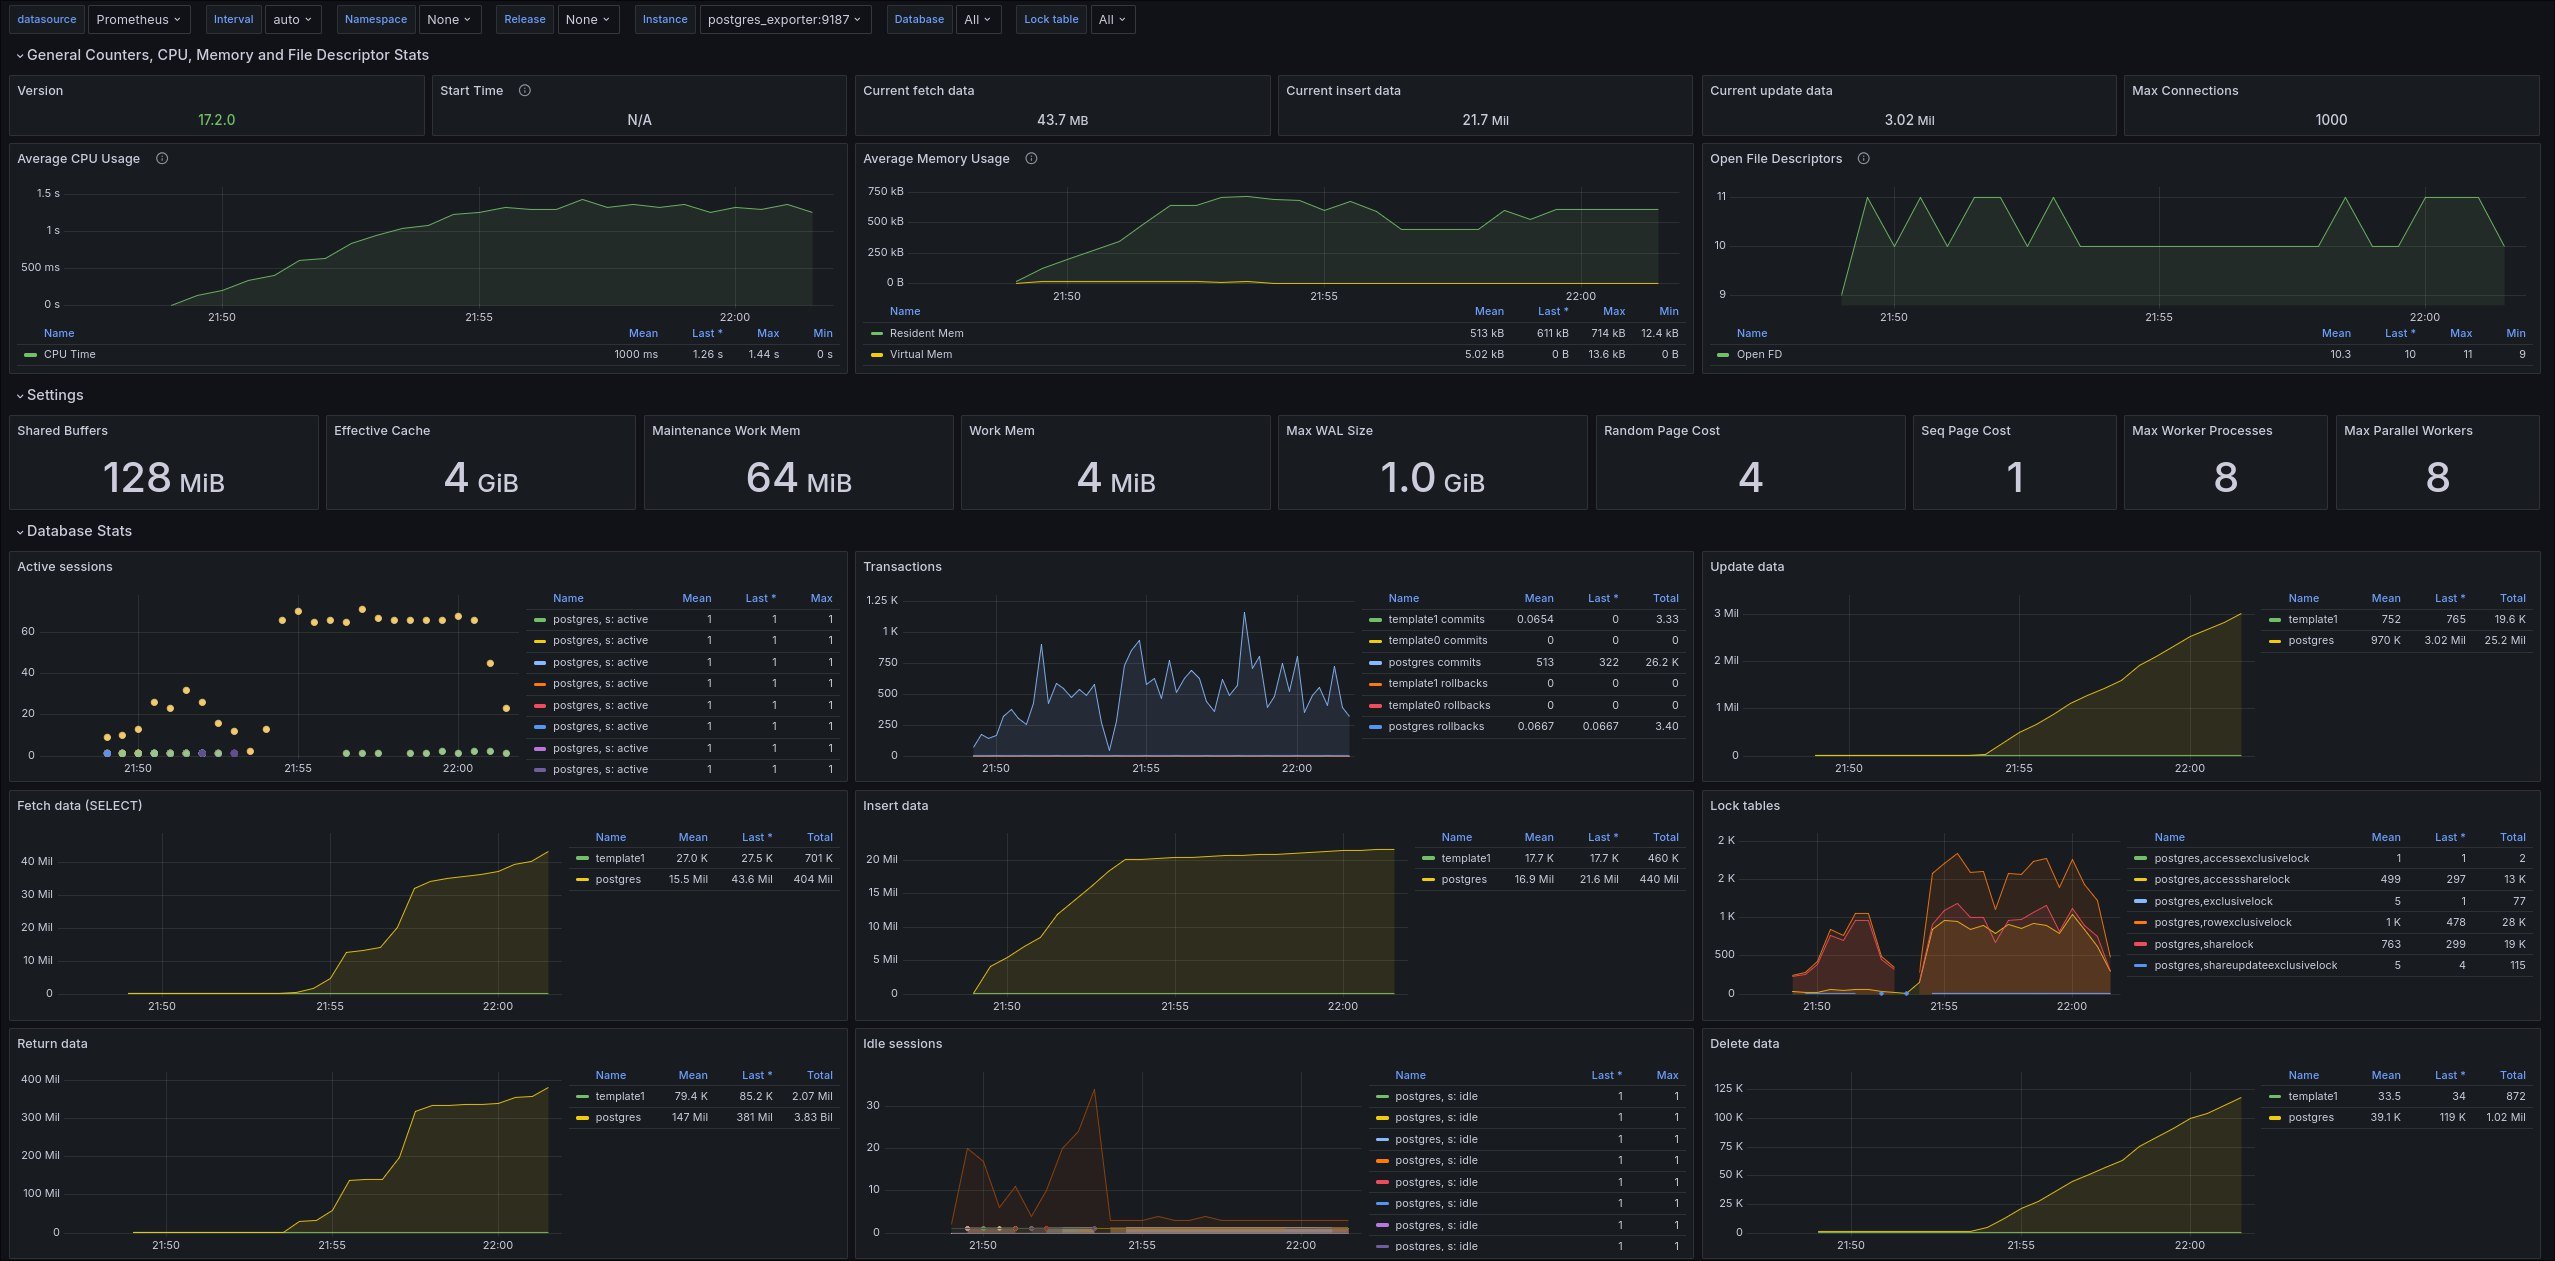
\includegraphics[width=0.8\textwidth]{imgs/citus.jpg}
	\caption{Resultados do TPC-C para o Citus}
	\label{fig:tpc-c}
\end{figure}

\begin{figure}[H]
	\centering
	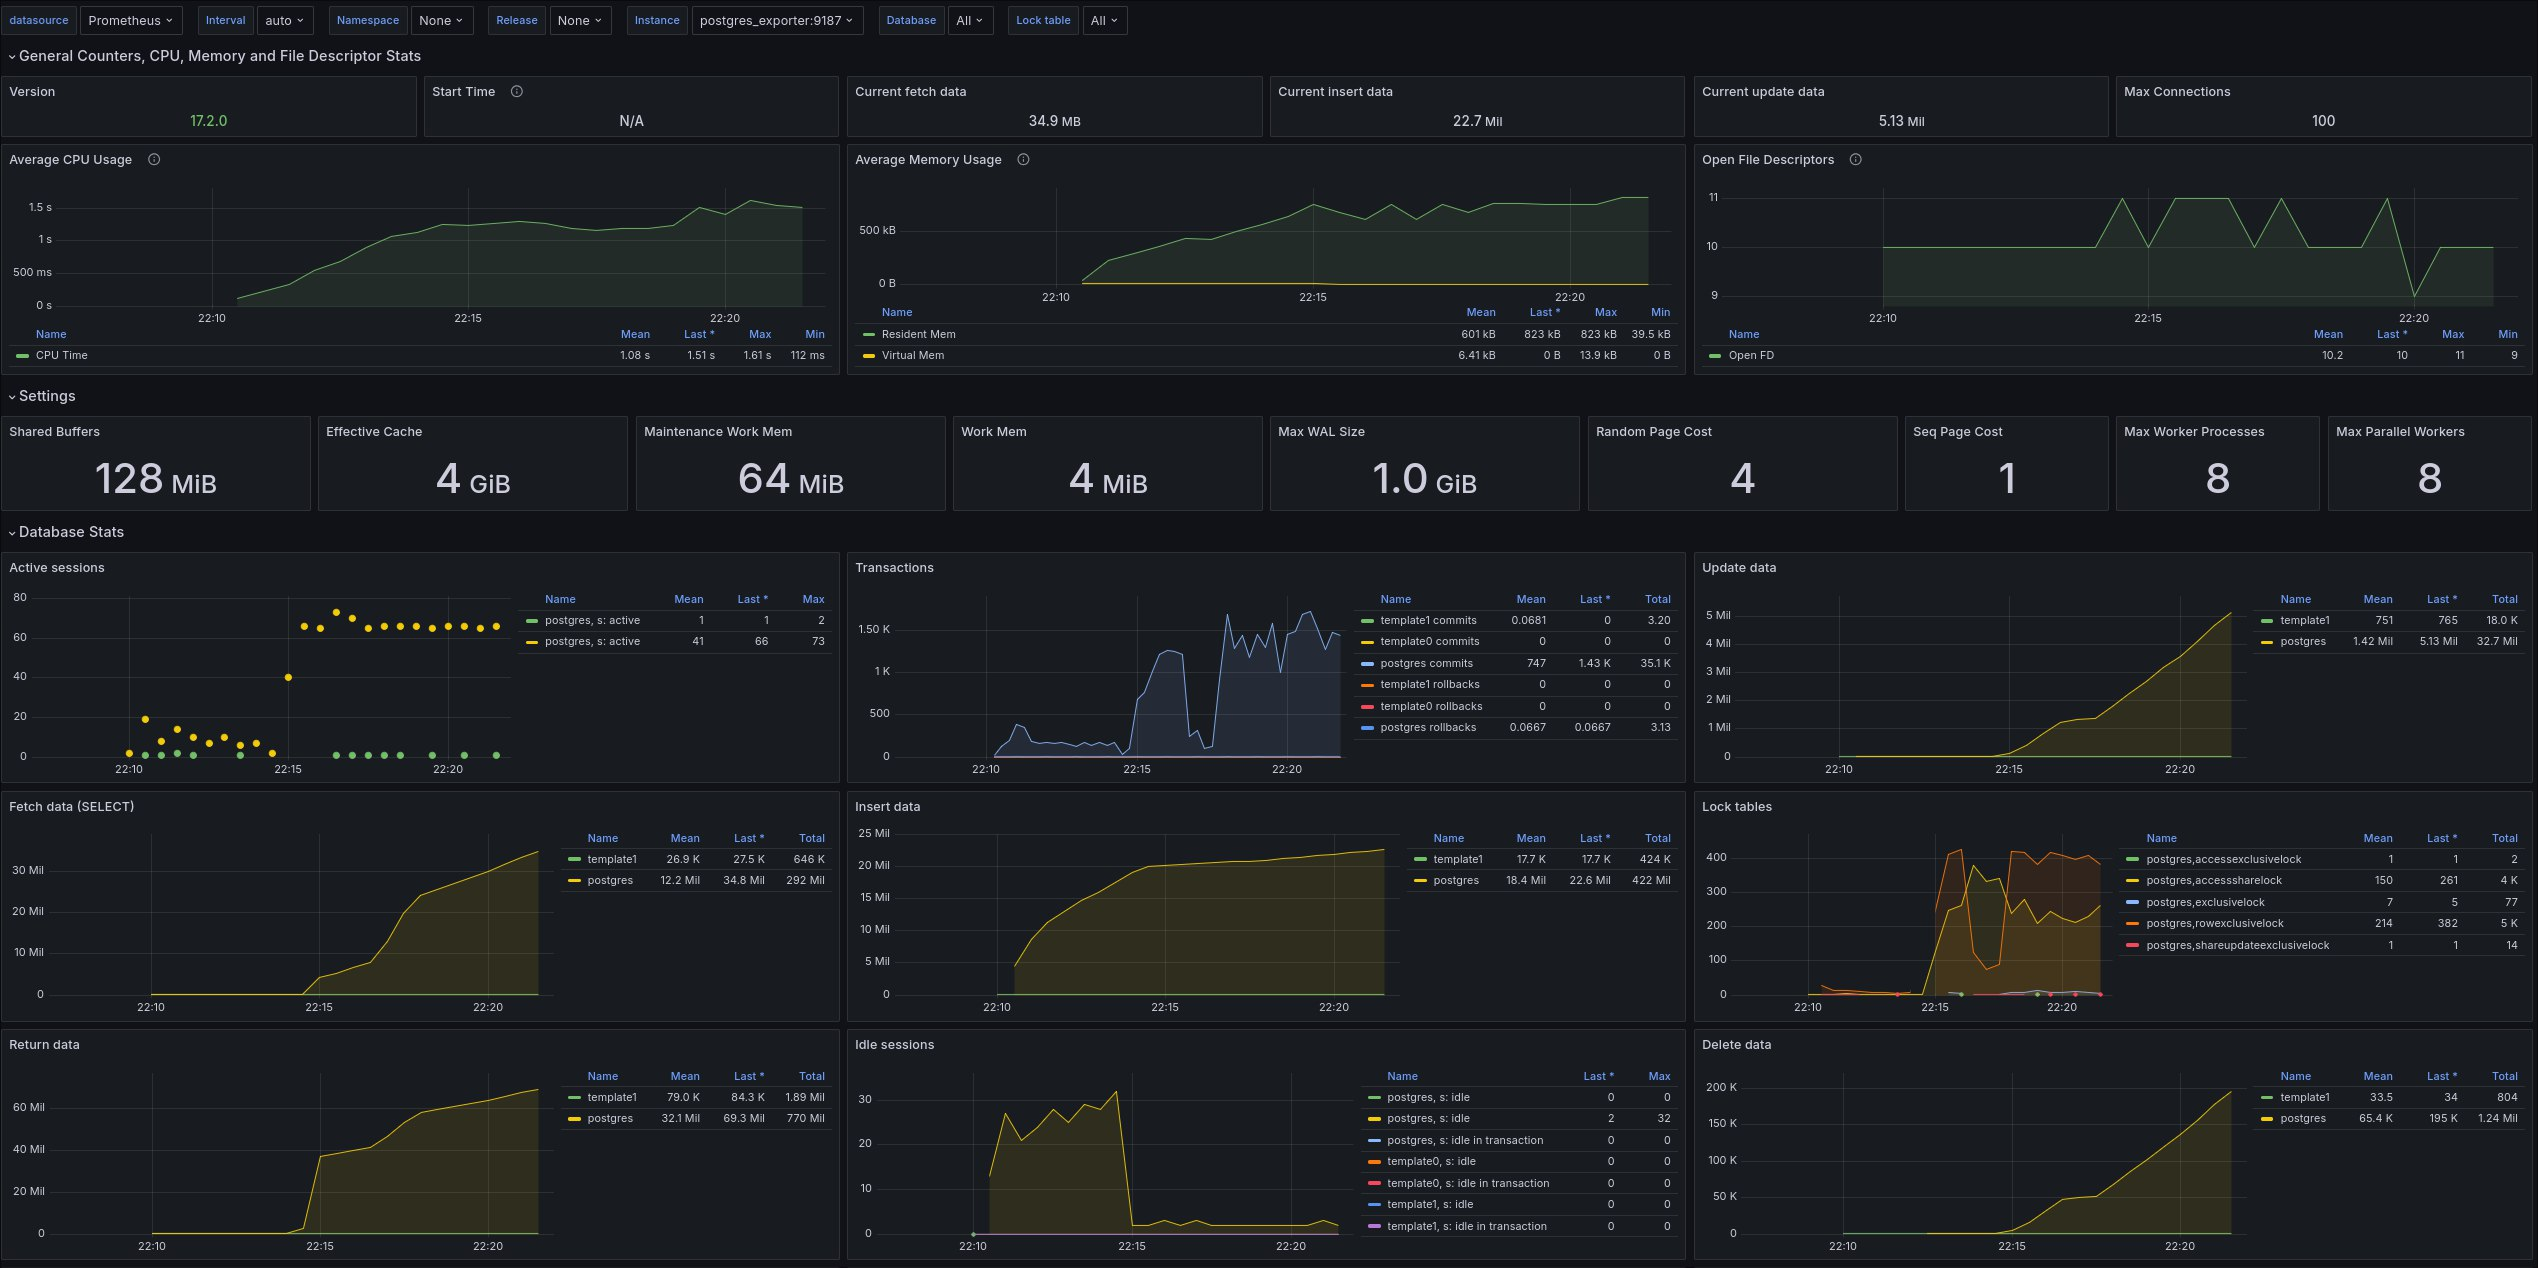
\includegraphics[width=0.8\textwidth]{imgs/Postgres.jpg}
	\caption{Resultados do TPC-C para o PostgreSQL}
	\label{fig:tpc-c}
\end{figure}

Como resultados, obtemos que O PostgreSQL atingiu 31405 operações novas por minuto e 72424 transações por minuto, 
enquanto o Citus atingiu 15304 operações novas por minuto e 35762 transações por minuto.
Além disso, o tempo das operações está registrado nas tabelas a seguir:
